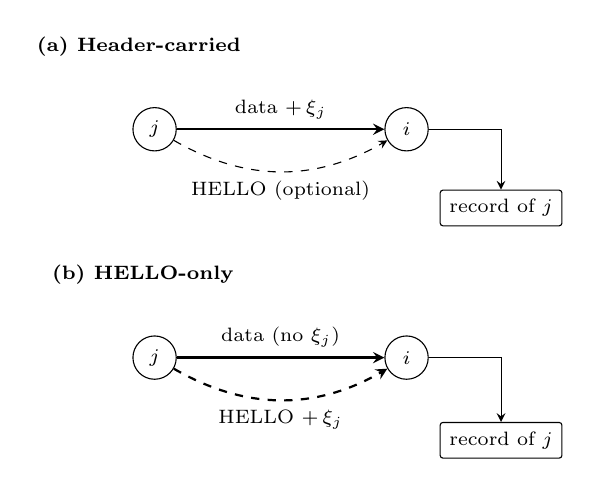
\begin{tikzpicture}[font=\scriptsize,>=stealth,node distance=0.5cm,
 nd/.style={circle,draw,minimum size=0.55cm,inner sep=0pt},
 tb/.style={draw,rounded corners=1pt,minimum width=1.5cm,minimum height=0.45cm,align=center}]
% panel a
\node[font=\scriptsize\bfseries] at (-0.2,2.55) {(a) Header-carried};
\node[nd] (a1) at (0,1.5) {$j$};
\node[nd] (a2) at (3.2,1.5) {$i$};
\draw[->,thick] (a1) -- node[above,pos=.5]{data $+\,\xi_j$} (a2);
\draw[->,dashed] (a1) to[bend right=30] node[below,pos=.5]{HELLO (optional)} (a2);
\node[tb] (ta) at (4.4,0.5) {record of $j$};
\draw[->] (a2) -| (ta);
% panel b
\node[font=\scriptsize\bfseries] at (-0.15,-0.35) {(b) HELLO-only};
\node[nd] (b1) at (0,-1.4) {$j$};
\node[nd] (b2) at (3.2,-1.4) {$i$};
\draw[->,thick] (b1) -- node[above,pos=.5]{data (no $\xi_j$)} (b2);
\draw[->,dashed,thick] (b1) to[bend right=30] node[below]{HELLO $+\,\xi_j$} (b2);
\node[tb] (tb) at (4.4,-2.45) {record of $j$};
\draw[->] (b2) -| (tb);
\end{tikzpicture}
